\documentclass[journal, onecolumn]{IEEEtran}

% ─── Packages ────────────────────────────────────────────────────────────────
\usepackage[T1]{fontenc}
\usepackage[utf8]{inputenc}
\usepackage[pdftex]{graphicx}
\usepackage{amsmath,amssymb}
\usepackage{array}
\usepackage{booktabs}
\usepackage{url}
\usepackage{hyperref}
\usepackage{xcolor}
\usepackage{listings}
\usepackage{tikz}
\usepackage{caption}
\usepackage{subcaption}
\usepackage{float}
\usepackage{multirow}
\usepackage{geometry}
\usepackage{mdframed}
\usepackage{tabularx}
\usepackage{colortbl}

\usetikzlibrary{shapes.geometric, arrows.meta, positioning, backgrounds}

\geometry{margin=1in}

% ─── Graphics path ───────────────────────────────────────────────────────────
\graphicspath{{report_images/}}
\DeclareGraphicsExtensions{.jpg,.jpeg,.png,.pdf}

% ─── Listing style ────────────────────────────────────────────────────────────
\definecolor{codebg}{RGB}{248,248,248}
\definecolor{codeframe}{RGB}{200,200,200}
\definecolor{keywordcolor}{RGB}{0,0,180}
\definecolor{commentcolor}{RGB}{80,130,80}
\definecolor{stringcolor}{RGB}{163,21,21}

\lstdefinestyle{pythonstyle}{
  language=Python,
  backgroundcolor=\color{codebg},
  frame=single,
  rulecolor=\color{codeframe},
  basicstyle=\ttfamily\footnotesize,
  keywordstyle=\color{keywordcolor}\bfseries,
  commentstyle=\color{commentcolor}\itshape,
  stringstyle=\color{stringcolor},
  numberstyle=\tiny\color{gray},
  numbers=left,
  stepnumber=1,
  numbersep=8pt,
  showspaces=false,
  showstringspaces=false,
  breaklines=true,
  breakatwhitespace=true,
  tabsize=4,
  captionpos=b,
}
\lstset{style=pythonstyle}

% ─── TikZ styles ──────────────────────────────────────────────────────────────
\tikzset{
  hw/.style   ={rectangle, rounded corners=4pt, draw=blue!60,  fill=blue!8,
                text centered, minimum width=2.1cm, minimum height=1.0cm,
                font=\small\bfseries, text width=2.0cm},
  sw/.style   ={rectangle, rounded corners=4pt, draw=orange!70, fill=orange!8,
                text centered, minimum width=2.0cm, minimum height=0.9cm,
                font=\small\bfseries},
  io/.style   ={rectangle, rounded corners=4pt, draw=green!60!black, fill=green!8,
                text centered, minimum width=2.0cm, minimum height=0.9cm,
                font=\small\bfseries},
  pipe/.style ={-Stealth, thick, draw=gray!60},
}

% ─── Hyperref ─────────────────────────────────────────────────────────────────
\hypersetup{colorlinks=true, linkcolor=blue!70!black, citecolor=green!50!black,
            urlcolor=blue!70!black}

% ─── Info box ─────────────────────────────────────────────────────────────────
\newmdenv[backgroundcolor=blue!4, linecolor=blue!40, linewidth=1pt,
          innerleftmargin=8pt, innerrightmargin=8pt,
          innertopmargin=5pt, innerbottommargin=5pt]{infobox}

\hyphenation{op-tical Hailo semi-conduc-tor}

% =============================================================================
%  TITLE & AUTHORS
% =============================================================================
\begin{document}

\title{Edge AI Based Hailo-Accelerated Real-Time 2D Semantic Mapping\\
       with RPi5 for Assistive Navigation}

\author{Karney Jayanath,~\textit{SR~26831},\quad
        Shreevathsa~K~S,~\textit{SR~25905},\quad
        Rajneesh Babu,~\textit{SR~26058}\\[2pt]
        \textit{CP330 — Edge AI, Department of Computational and Data Sciences,}\\
        \textit{Indian Institute of Science (IISc), Bengaluru}\\
        \textit{Instructor: Dr.\ Pandarasamy Arjunan} \quad|\quad \textit{May 2026}
}

\markboth{CP330 — Edge AI, IISc, May 2026}{}
\maketitle

% =============================================================================
\begin{abstract}
This paper presents a real-time semantic navigation aid for visually impaired (VI) users built on a \textbf{Raspberry Pi 5} and \textbf{Hailo-8 AI HAT} (13\,TOPS NPU). A Pi Camera captures live 640$\times$480 video; a pruned, INT8-quantized YOLOv8n model compiled to Hailo Executable Format (HEF) detects up to 20 indoor-relevant object classes at \textbf{24.7\,FPS}. An Arduino Nicla Vision module streams gyroscope yaw over USB, which is fused with per-frame bounding-box detections to build a persistent \textbf{2D polar semantic map} displayed in a live OpenCV window. The system outputs two simultaneous display windows: a detection feed with labeled bounding boxes and a top-down map showing object positions relative to the user. A five-stage model optimization pipeline (FP32 fine-tuning $\to$ PTQ $\to$ QAT $\to$ L1 pruning $\to$ Hailo HEF) achieves a \textbf{+9.4\% mAP50 gain} and \textbf{1.87$\times$ speed-up} over the uncompressed baseline, while reducing the deployable model to just \textbf{4.5\,MB}.
\end{abstract}

\begin{IEEEkeywords}
Edge AI, YOLOv8, INT8 Quantization, Structured Pruning, Hailo-8 NPU,
Raspberry Pi 5, Semantic Mapping, Assistive Navigation, Real-Time Object Detection
\end{IEEEkeywords}

% =============================================================================
\section{Introduction}
\label{sec:intro}
% =============================================================================

Assistive navigation for the visually impaired has traditionally relied on hardware such as white canes and GPS-based devices, which offer limited real-time situational awareness. With the rapid advancement of edge AI hardware, it is now possible to run deep-learning perception models on compact single-board computers at interactive frame rates, opening the door to richer, low-cost navigation aids.

The YOLO family of object detectors~\cite{redmon2016you,jocher2023yolov8} provides fast and accurate multi-class detection, but deploying these models on severely resource-constrained platforms requires careful compression. The \textbf{Hailo-8}~\cite{hailo8} accelerator delivers 13\,TOPS in an M.2 form factor and interfaces with the RPi5 over PCIe, but it requires models to be compiled into a proprietary \emph{Hailo Executable Format} (HEF) using the Hailo Dataflow Compiler (DFC). This compilation step introduces several non-trivial engineering challenges, particularly around YOLOv8's multi-head output structure.

Our system addresses the full end-to-end problem: training and compressing a YOLOv8n model on Google Colab, compiling it for the Hailo NPU, deploying it on the RPi5, and fusing the detections with IMU yaw to produce a live 2D map that an operator or carer can read at a glance.

The three main contributions of this work are:
\begin{enumerate}
  \item A reproducible five-stage compression pipeline from FP32 YOLOv8n to a 4.5\,MB Hailo HEF, benchmarked on COCO128.
  \item A custom Distribution Focal Loss (DFL) decoder that handles Hailo's six-head raw output format on the RPi5 CPU.
  \item A sensor-fused 2D semantic map that combines monocular bounding-box detections with gyroscope yaw to display object locations relative to the user in real time.
\end{enumerate}

% =============================================================================
\section{System Architecture}
\label{sec:arch}
% =============================================================================

\subsection{Hardware Setup}

The system integrates four components connected as shown in Table~\ref{tab:hw} and Figure~\ref{fig:arch}.

\begin{table}[H]
\centering
\caption{Hardware Components and Specifications}
\label{tab:hw}
\begin{tabular}{llll}
\toprule
\textbf{Component} & \textbf{Model} & \textbf{Role} & \textbf{Key Spec} \\
\midrule
Main compute     & Raspberry Pi 5       & Pre/post-processing, display   & Cortex-A76, 8\,GB RAM \\
AI accelerator   & Hailo-8 AI HAT       & YOLOv8n HEF inference          & 13\,TOPS, M.2 PCIe \\
Camera           & TNBA1392 (CSI)       & RGB frame capture              & 640$\times$480, 30\,FPS target \\
IMU sensor       & Arduino Nicla Vision & Gyroscope yaw over USB         & LSM6DSOX, 50\,Hz \\
\bottomrule
\end{tabular}
\end{table}

\noindent\textbf{Physical connections:}
The camera connects to RPi5's CAM0 port via CSI ribbon cable. The Hailo-8 AI HAT sits on top of the RPi5 via M.2/PCIe. The Nicla Vision connects to an RPi5 USB port via micro-USB and streams yaw angle data over USB serial at 115200\,baud. The whole system is powered by a USB-C power bank.

\subsection{Data Flow}

Figure~\ref{fig:arch} shows the six-stage per-frame pipeline. At approximately 25\,FPS, each frame is captured, resized, sent to the NPU, decoded, fused with the latest IMU yaw, and used to update both the detection display and the 2D semantic map.

\begin{figure}[H]
\centering
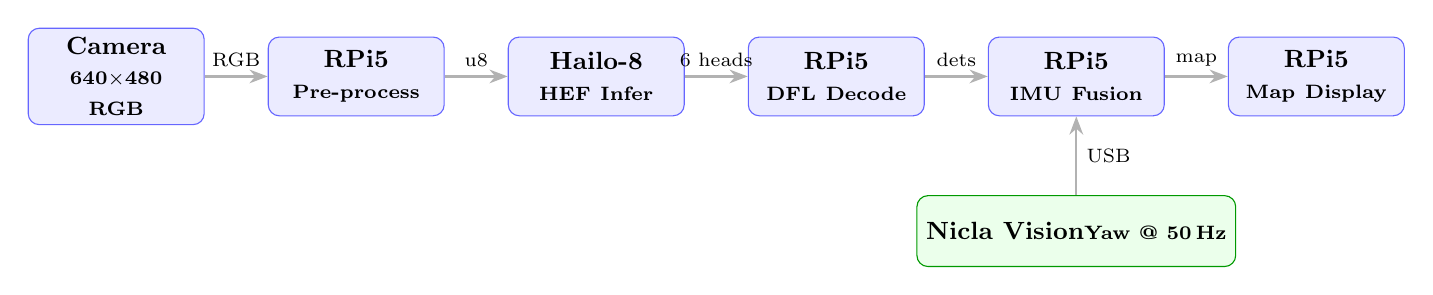
\begin{tikzpicture}[node distance=1.1cm, auto]

  \node[hw] (cam)    {Camera\\{\scriptsize 640$\times$480 RGB}};
  \node[hw, right=0.8cm of cam]  (pre)    {RPi5\\{\scriptsize Pre-process}};
  \node[hw, right=0.8cm of pre]  (hailo)  {Hailo-8\\{\scriptsize HEF Infer}};
  \node[hw, right=0.8cm of hailo](dfl)    {RPi5\\{\scriptsize DFL Decode}};
  \node[hw, right=0.8cm of dfl]  (fusion) {RPi5\\{\scriptsize IMU Fusion}};
  \node[hw, right=0.8cm of fusion](map)   {RPi5\\{\scriptsize Map Display}};
  \node[io, below=1.0cm of fusion](imu)   {Nicla Vision\\{\scriptsize Yaw @ 50\,Hz}};

  \draw[pipe] (cam)    -- node[above, font=\scriptsize]{RGB} (pre);
  \draw[pipe] (pre)    -- node[above, font=\scriptsize]{u8} (hailo);
  \draw[pipe] (hailo)  -- node[above, font=\scriptsize]{6 heads} (dfl);
  \draw[pipe] (dfl)    -- node[above, font=\scriptsize]{dets} (fusion);
  \draw[pipe] (fusion) -- node[above, font=\scriptsize]{map} (map);
  \draw[pipe] (imu)    -- node[right, font=\scriptsize]{USB} (fusion);

\end{tikzpicture}
\caption{Six-stage per-frame data flow. The Hailo-8 handles only NPU inference; all other computation runs on the RPi5 Cortex-A76 CPU.}
\label{fig:arch}
\end{figure}

\subsection{Output Windows}

The system produces two simultaneous OpenCV display windows on the RPi5:

\begin{enumerate}
  \item \textbf{Detection window} — live camera feed with labeled bounding boxes, confidence scores, and an FPS/IMU overlay at the top.
  \item \textbf{2D Semantic Map} — a top-down polar map centered on the user, showing each detected object as a colored dot at its estimated distance and heading angle. Range rings are drawn at 1\,m intervals up to 6\,m; color encodes proximity (orange $<$2.5\,m, green $\geq$2.5\,m).
\end{enumerate}

There is \emph{no audio or voice output} in the current implementation. All feedback is visual.

\subsection{Detection Classes}

Twenty COCO classes relevant to indoor navigation were selected, discarding classes such as vehicles, animals, and outdoor objects. The retained classes are listed in Table~\ref{tab:classes}.

\begin{table}[H]
\centering
\caption{Twenty VI-Relevant Detection Classes (COCO IDs)}
\label{tab:classes}
\begin{tabular}{llllll}
\toprule
person (0) & backpack (24) & handbag (26) & suitcase (28) & bottle (39) & cup (41) \\
fork (42)  & knife (43)    & spoon (44)   & bowl (45)     & chair (56)  & couch (57) \\
bed (59)   & dining table (60) & laptop (63) & mouse (64) & remote (65) & keyboard (66) \\
cell phone (67) & book (73) & & & & \\
\bottomrule
\end{tabular}
\end{table}

% =============================================================================
\section{Model Optimization Pipeline}
\label{sec:opt}
% =============================================================================

Starting from a pretrained YOLOv8n checkpoint, we applied a five-stage pipeline to compress the model for Hailo-8 deployment. All training and compilation run on Google Colab (T4 GPU for training; CPU-only for HEF compilation due to Blackwell GPU incompatibility with the DFC).

\subsection{Stage 1 — FP32 Baseline Fine-Tuning}

YOLOv8n was fine-tuned for 20 epochs on COCO128, restricted to the 20 target class IDs.

\begin{lstlisting}[caption={Baseline fine-tuning on Colab T4},label=lst:train]
from ultralytics import YOLO

TARGET_CLASS_IDS = [0,24,26,28,39,41,42,43,44,45,
                    56,57,59,60,63,64,65,66,67,73]
model = YOLO('yolov8n.pt')
model.train(data='coco128.yaml', epochs=20,
            imgsz=640, batch=16, device=0,
            classes=TARGET_CLASS_IDS, name='baseline_v8n')
\end{lstlisting}

\noindent\textbf{Result:} mAP50 = 0.6269, latency = 8.30\,ms, size = 6.23\,MB.

\subsection{Stage 2 — Post-Training Quantization (PTQ, TensorRT INT8)}

PTQ converts the FP32 weights to INT8 using 64 COCO128 calibration images, with no retraining. Ultralytics' built-in TensorRT INT8 export correctly handles YOLOv8's output heads.

\noindent\textbf{Result:} mAP50 = 0.6093 ($-$2.8\%), latency = 4.66\,ms (1.78$\times$ faster).

\subsection{Stage 3 — Quantization-Aware Training (QAT)}

QAT retrains the model for 20 epochs with quantization noise injected during the forward pass, so weights adapt to INT8 precision before export. The model was then exported to TensorRT INT8.

\noindent\textbf{Result:} mAP50 = 0.5944 ($-$5.2\% vs.\ baseline). The accuracy drop is expected because COCO128 is too small for QAT; a full COCO training set would be needed for QAT to be effective.

\subsection{Stage 4 — Structured L1 Pruning + Fine-Tuning}

Structured pruning removes entire convolutional filters ranked lowest by L1-norm. Unlike weight-level sparsity, filter removal produces a genuinely smaller and faster dense model with no sparse-matrix overhead.

\begin{lstlisting}[caption={L1 filter pruning applied to all Conv2d layers},label=lst:prune]
import torch.nn.utils.prune as prune

for name, module in model.named_modules():
    if isinstance(module, torch.nn.Conv2d):
        prune.l1_unstructured(
            module, name='weight', amount=0.2)
        prune.remove(module, 'weight')
\end{lstlisting}

After pruning, the model was fine-tuned for 20 more epochs to recover accuracy, then exported to TensorRT INT8.

\noindent\textbf{Result:} mAP50 = \textbf{0.6793} — the best across all stages. Removing noisy low-magnitude filters before quantization acts as implicit regularization. Latency = 4.58\,ms, size = 5.65\,MB.

\subsection{Stage 5 — Knowledge Distillation (Ablation Only)}

A YOLOv8s teacher generated pseudo-labels on COCO128; the pruned YOLOv8n student was trained on these labels. This is a response-based KD approach (Born-Again Networks).

\noindent\textbf{Result:} mAP50 = 0.5904 ($-$4.86\% vs.\ baseline). KD underperformed on this small dataset and was \emph{not included} in the final pipeline. It is reported here as an ablation.

\subsection{Stage 6 — Hailo HEF Compilation}

The pruned INT8 model was exported to ONNX (opset 11) and compiled using DFC v3.33.1 in three steps:
\begin{enumerate}
  \item \textbf{Parse}: ONNX $\to$ HAR (Hailo Archive) — DFC reads the graph.
  \item \textbf{Optimize}: INT8 calibration using 64 COCO128 images.
  \item \textbf{Compile}: HAR $\to$ HEF — operations mapped across 8 Hailo clusters.
\end{enumerate}

\begin{infobox}
\textbf{Engineering Note — 6-head Detect split.}
YOLOv8's Detect module produces 6 raw output tensors (3 box + 3 class, one per feature-map scale at strides 8/16/32). The DFC cannot absorb the DFL softmax-expectation step, so the HEF outputs all 6 raw tensors and the DFL decoding runs on the RPi5 CPU after every inference call.
\end{infobox}

\noindent\textbf{Result:} HEF size = \textbf{4.50\,MB}, all 8 Hailo clusters utilized.

\subsection{Pipeline Summary}

\begin{table}[H]
\centering
\caption{Optimization Pipeline Benchmark — COCO128 Validation Set}
\label{tab:benchmark}
\begin{tabular}{lcccc}
\toprule
\textbf{Stage} & \textbf{mAP50} & \textbf{FPS (T4)} & \textbf{Latency (ms)} & \textbf{Size (MB)} \\
\midrule
Baseline FP32                        & 0.6269 & 120.5 & 8.30 & 6.23 \\
PTQ INT8                             & 0.6093 & 214.4 & 4.66 & 5.57 \\
QAT INT8                             & 0.5944 & 186.6 & 5.36 & 5.65 \\
\rowcolor{green!15}
Pruned INT8 \textbf{(deployed)}      & \textbf{0.6793} & \textbf{218.3} & \textbf{4.58} & 5.65 \\
KD INT8 (ablation)                   & 0.5904 & 120.5 & 8.30 & 6.23 \\
\midrule
Hailo HEF on RPi5                    & —      & 24.7  & 40.5 & \textbf{4.50} \\
\bottomrule
\end{tabular}
\end{table}

The pruned model achieves \textbf{+9.4\% mAP50} over the FP32 baseline while running \textbf{1.87$\times$ faster} on the Colab T4.

\begin{figure}[H]
\centering
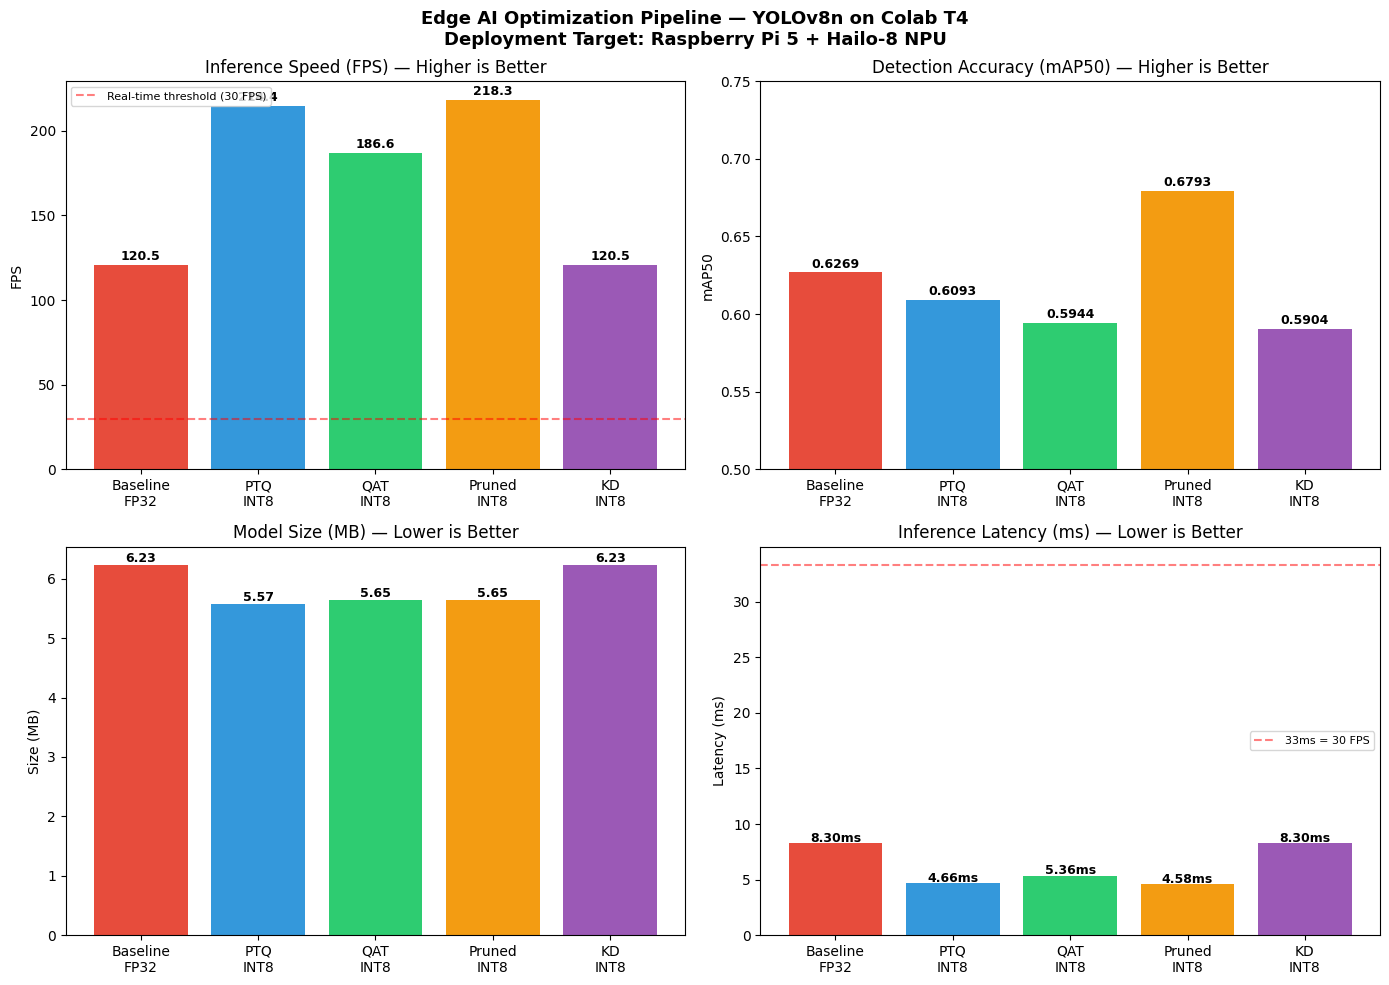
\includegraphics[width=0.90\textwidth]{comparison_chart}
\caption{Four-panel benchmark comparison across all optimization stages: FPS (top-left), mAP50 (top-right), model size in MB (bottom-left), and inference latency in ms (bottom-right). All benchmarks are on Colab T4 GPU; the Hailo-8 on-device figures are reported separately in Table~\ref{tab:perf}.}
\label{fig:chart}
\end{figure}

% =============================================================================
\section{Implementation}
\label{sec:impl}
% =============================================================================

\subsection{Implementation Overview}

The full project is divided into three independent workstreams that come together on the RPi5 at runtime. Figure~\ref{fig:impl_flow} shows the end-to-end implementation flow.

\begin{figure}[H]
\centering
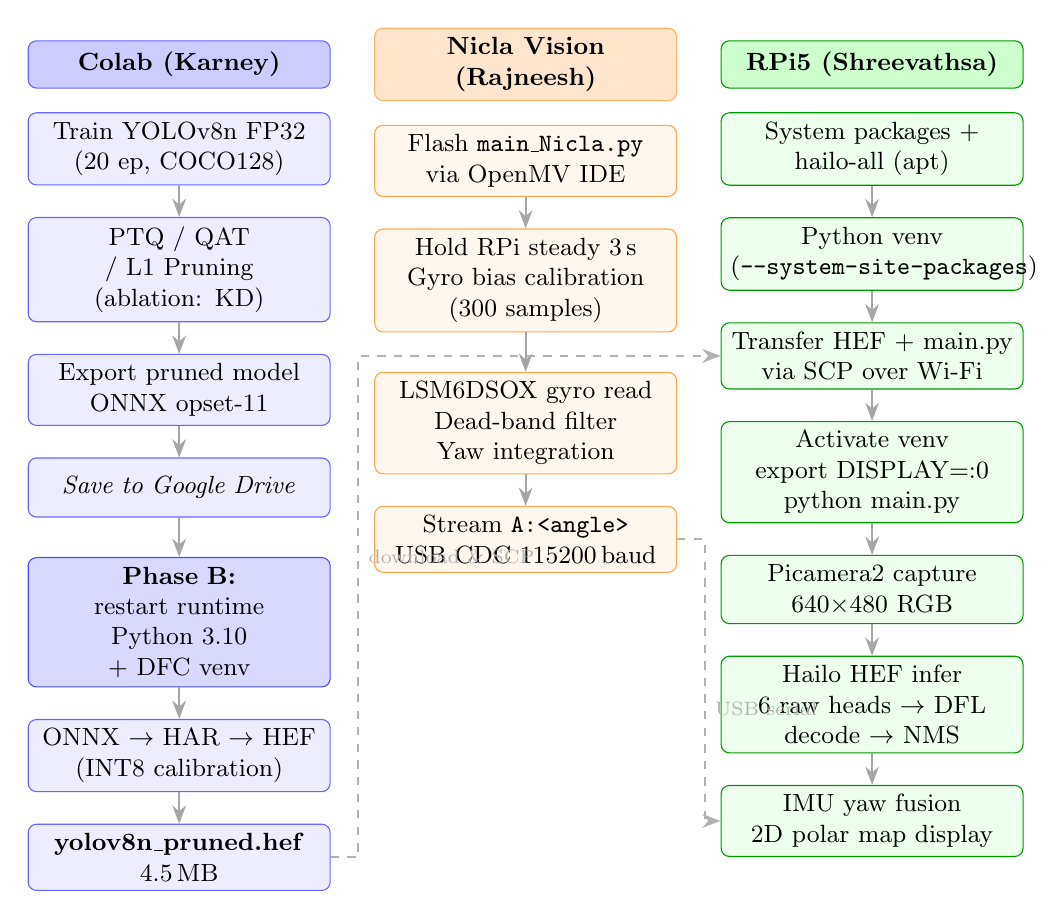
\begin{tikzpicture}[node distance=0.5cm and 0.6cm]

  % ── Column styles ──────────────────────────────────────────────────
  \tikzset{
    colA/.style={rectangle, rounded corners=3pt, draw=blue!60, fill=blue!7,
                 text width=3.6cm, minimum height=0.75cm, text centered, font=\small},
    colB/.style={rectangle, rounded corners=3pt, draw=orange!70, fill=orange!7,
                 text width=3.6cm, minimum height=0.75cm, text centered, font=\small},
    colC/.style={rectangle, rounded corners=3pt, draw=green!60!black, fill=green!7,
                 text width=3.6cm, minimum height=0.75cm, text centered, font=\small},
    hdr/.style={rectangle, rounded corners=3pt, text width=3.6cm, minimum height=0.6cm,
                text centered, font=\small\bfseries},
    arr/.style={-Stealth, thick, gray!70},
    sarr/.style={-Stealth, thick, dashed, gray!60},
  }

  % ── Column headers ─────────────────────────────────────────────────
  \node[hdr, fill=blue!20,  draw=blue!60]   (hA) at (0,0)   {Colab (Karney)};
  \node[hdr, fill=orange!20,draw=orange!60] (hB) at (4.4,0) {Nicla Vision (Rajneesh)};
  \node[hdr, fill=green!20, draw=green!60!black] (hC) at (8.8,0) {RPi5 (Shreevathsa)};

  % ── Column A — Colab ───────────────────────────────────────────────
  \node[colA, below=0.3cm of hA]  (a1) {Train YOLOv8n FP32\\(20 ep, COCO128)};
  \node[colA, below=0.4cm of a1]  (a2) {PTQ / QAT / L1 Pruning\\(ablation: KD)};
  \node[colA, below=0.4cm of a2]  (a3) {Export pruned model\\ONNX opset-11};
  \node[colA, below=0.4cm of a3]  (a4) {\textit{Save to Google Drive}};
  \node[colA, below=0.5cm of a4, fill=blue!15, draw=blue!70] (a5)
        {\textbf{Phase B:} restart runtime\\Python 3.10 + DFC venv};
  \node[colA, below=0.4cm of a5]  (a6) {ONNX $\to$ HAR $\to$ HEF\\(INT8 calibration)};
  \node[colA, below=0.4cm of a6]  (a7) {\textbf{yolov8n\_pruned.hef}\\4.5\,MB};

  \draw[arr] (a1)--(a2); \draw[arr] (a2)--(a3);
  \draw[arr] (a3)--(a4); \draw[arr] (a4)--(a5);
  \draw[arr] (a5)--(a6); \draw[arr] (a6)--(a7);

  % ── Column B — Nicla ───────────────────────────────────────────────
  \node[colB, below=0.3cm of hB]  (b1) {Flash \texttt{main\_Nicla.py}\\via OpenMV IDE};
  \node[colB, below=0.4cm of b1]  (b2) {Hold RPi steady 3\,s\\Gyro bias calibration\\(300 samples)};
  \node[colB, below=0.5cm of b2]  (b3) {LSM6DSOX gyro read\\Dead-band filter\\Yaw integration};
  \node[colB, below=0.4cm of b3]  (b4) {Stream \texttt{A:<angle>}\\USB CDC 115200\,baud};

  \draw[arr] (b1)--(b2); \draw[arr] (b2)--(b3); \draw[arr] (b3)--(b4);

  % ── Column C — RPi5 ────────────────────────────────────────────────
  \node[colC, below=0.3cm of hC]  (c1) {System packages +\\hailo-all (apt)};
  \node[colC, below=0.4cm of c1]  (c2) {Python venv\\(\texttt{--system-site-packages})};
  \node[colC, below=0.4cm of c2]  (c3) {Transfer HEF + main.py\\via SCP over Wi-Fi};
  \node[colC, below=0.4cm of c3]  (c4) {Activate venv\\export DISPLAY=:0\\python main.py};
  \node[colC, below=0.4cm of c4]  (c5) {Picamera2 capture\\640$\times$480 RGB};
  \node[colC, below=0.4cm of c5]  (c6) {Hailo HEF infer\\6 raw heads $\to$ DFL decode $\to$ NMS};
  \node[colC, below=0.4cm of c6]  (c7) {IMU yaw fusion\\2D polar map display};

  \draw[arr] (c1)--(c2); \draw[arr] (c2)--(c3); \draw[arr] (c3)--(c4);
  \draw[arr] (c4)--(c5); \draw[arr] (c5)--(c6); \draw[arr] (c6)--(c7);

  % ── Cross-column arrows ────────────────────────────────────────────
  % HEF from Colab to RPi5
  \draw[sarr] (a7.east) -- ++(0.35,0) |- node[right, font=\scriptsize, pos=0.3]
              {download \& SCP} (c3.west);
  % IMU stream from Nicla to RPi5
  \draw[sarr] (b4.east) -- ++(0.35,0) |- node[right, font=\scriptsize, pos=0.3]
              {USB serial} (c7.west);

\end{tikzpicture}
\caption{End-to-end implementation flow across the three workstreams. Dashed arrows show artifact/data handoffs between workstreams: the compiled HEF is transferred to the RPi5 via SCP; the Nicla Vision streams yaw over USB serial to the RPi5 at runtime.}
\label{fig:impl_flow}
\end{figure}

% ─────────────────────────────────────────────────────────────────────────────
\subsection{Phase A — Model Training and ONNX Export (Colab T4)}
\label{sec:phaseA}
% ─────────────────────────────────────────────────────────────────────────────

All training and optimization runs on a standard Colab T4 GPU runtime. After the five optimization stages described in Section~\ref{sec:opt}, the best-performing pruned model is exported to ONNX with opset version 11 and saved to Google Drive.

\begin{lstlisting}[caption={Export pruned model to opset-11 ONNX for DFC compatibility},label=lst:onnx]
from ultralytics import YOLO

model = YOLO('/content/runs/detect/pruned_v8n/weights/best.pt')
model.export(format='onnx', imgsz=640, opset=11,
             simplify=True)
# Saved to: best_opset11.onnx (~12 MB)
\end{lstlisting}

\noindent Opset 11 is required because the Hailo DFC does not support several operators introduced in opset 13 (the Ultralytics default). The ONNX model and the Hailo DFC \texttt{.whl} installer are both uploaded to Google Drive before restarting the runtime.

% ─────────────────────────────────────────────────────────────────────────────
\subsection{Phase B — HEF Compilation (Colab, Separate Runtime)}
\label{sec:phaseB}
% ─────────────────────────────────────────────────────────────────────────────

HEF compilation is done in a separate Colab session because the Hailo Dataflow Compiler (DFC v3.33.1) requires Python 3.10 and a specific numpy version, and the DFC \texttt{optimize} step is incompatible with Colab's NVIDIA Blackwell CUDA libraries. The workaround is to force CPU-only mode.

\textbf{Setup steps after restarting runtime:}
\begin{enumerate}
  \item Mount Google Drive and load \texttt{best\_opset11.onnx} and the DFC \texttt{.whl}.
  \item Create a Python 3.10 virtual environment and install the DFC wheel.
  \item Run the three-step compilation: \textbf{Parse} (ONNX $\to$ HAR), \textbf{Optimize} (INT8 calibration with 64 COCO128 images, CPU-only flag), \textbf{Compile} (HAR $\to$ HEF).
  \item Download the output \texttt{yolov8n\_pruned.hef} (4.5\,MB).
\end{enumerate}

The DFC \texttt{.whl} file must be downloaded manually from the Hailo Developer Zone: \textit{Accelerators $\to$ Hailo-8/8L $\to$ AI Software Suite $\to$ Dataflow Compiler $\to$ x86 / Linux / Python 3.10}.

\begin{infobox}
\textbf{Why 6 output heads?} YOLOv8's Detect module produces 3 box tensors (channels = 64 = $4 \times 16$ DFL bins) and 3 class tensors (channels = 80) — one pair per feature-map stride (8, 16, 32). The DFC cannot fuse the DFL softmax-expectation into the HEF graph, so all 6 raw tensors are exported and decoded on the RPi5 CPU after every inference call.
\end{infobox}

% ─────────────────────────────────────────────────────────────────────────────
\subsection{Nicla Vision — IMU Firmware and Yaw Streaming}
\label{sec:nicla}
% ─────────────────────────────────────────────────────────────────────────────

The Arduino Nicla Vision is programmed using OpenMV IDE (MicroPython). The firmware file \texttt{main\_Nicla.py} is copied to the Nicla's internal storage, renamed to \texttt{main.py}, and run via the IDE. Once verified, the Nicla is disconnected from the laptop and plugged into an RPi5 USB port.

\textbf{Startup calibration:} On boot, the LSM6DSOX gyroscope $z$-axis (yaw rate) is sampled 300 times at 10\,ms intervals ($\approx$3\,s). The mean is stored as a static bias $b_\psi$. The device must be held still and vertical during this window.

\textbf{Dead-band filter:} Small residual gyro noise at rest is suppressed:
\begin{equation}
  \dot{\psi}_\text{corrected} = \begin{cases}
    \dot{\psi} - b_\psi & \text{if } |\dot{\psi} - b_\psi| \geq 0.8\,^\circ\!/\text{s} \\
    0 & \text{otherwise}
  \end{cases}
\end{equation}

\textbf{Yaw integration:} The corrected angular rate is integrated at 50\,Hz to give a cumulative heading angle:
\begin{equation}
  \psi_t = \bigl(\psi_{t-1} + \dot{\psi}_\text{corrected} \cdot \Delta t\bigr) \bmod 360^\circ
\end{equation}

Each angle is sent to the RPi5 over USB CDC (115200\,baud) as \texttt{A:<angle>$\backslash$n}. The RPi5 reads from \texttt{/dev/ttyACM0} in a dedicated background thread, so the IMU never blocks the inference loop.

% ─────────────────────────────────────────────────────────────────────────────
\subsection{RPi5 — Setup and Inference Pipeline}
\label{sec:rpi5}
% ─────────────────────────────────────────────────────────────────────────────

\textbf{One-time setup} is done over SSH (laptop and RPi5 on the same Wi-Fi network):

\begin{lstlisting}[caption={RPi5 system package and Hailo runtime installation},label=lst:setup,language=bash]
# System packages
sudo apt install -y python3-venv python3-numpy python3-opencv \
  python3-serial python3-picamera2 v4l-utils rpicam-apps

# Hailo runtime (HailoRT + PCIe driver)
sudo apt install -y hailo-all

# Python virtual environment (needed because RPi OS
# blocks direct pip install)
cd ~/edge_nav
python3 -m venv venv_edge_nav --system-site-packages
source ~/edge_nav/venv_edge_nav/bin/activate
\end{lstlisting}

\textbf{File transfer:} The HEF and the inference script are copied from a Windows laptop to the RPi5 via SCP over Wi-Fi:

\begin{lstlisting}[caption={SCP transfer of HEF and inference script to RPi5},label=lst:scp,language=bash]
# Run in Windows PowerShell (replace <RPI_IP> with actual IP)
scp "$env:USERPROFILE\Downloads\yolov8n_pruned.hef" `
    rpi15@<RPI_IP>:/home/rpi15/edge_nav/models/
scp "$env:USERPROFILE\Downloads\main.py" `
    rpi15@<RPI_IP>:/home/rpi15/edge_nav/
\end{lstlisting}

\textbf{Running the system:}

\begin{lstlisting}[caption={Launching the inference and mapping system on RPi5},label=lst:run,language=bash]
cd ~/edge_nav
source ~/edge_nav/venv_edge_nav/bin/activate
export DISPLAY=:0
python main.py
\end{lstlisting}

\textbf{Hailo inference:} Each frame is resized to 640$\times$640, converted to RGB, and sent as a uint8 tensor to the Hailo-8 via HailoRT over PCIe. The NPU returns 6 raw float32 tensors.

\textbf{DFL Decoding:} A custom \texttt{YOLOv8DFLDecoder} class reconstructs bounding boxes from the 6 raw heads. For each of the 3 feature-map scales (stride $s \in \{8, 16, 32\}$):

\begin{equation}
  \text{dist}_{i} = \sum_{k=0}^{15} k \cdot \text{softmax}(\text{raw\_box}_{i,k}), \quad i \in \{x_1, y_1, x_2, y_2\}
  \label{eq:dfl}
\end{equation}
\begin{align}
  x_1 &= (c_x + 0.5)\cdot s \;-\; \text{dist}_{x_1} \cdot s \\
  x_2 &= (c_x + 0.5)\cdot s \;+\; \text{dist}_{x_2} \cdot s
\end{align}

Class scores are recovered via sigmoid: $p = \sigma(\text{raw\_cls})$. After decoding all three scales, class-wise NMS is applied (confidence $> 0.40$, IoU $< 0.45$) and only the 20 VI-relevant classes are kept.

\begin{lstlisting}[caption={DFL decode for one feature-map scale (core logic)},label=lst:dfl]
def decode_one_scale(box_raw, cls_raw, grid, stride):
    # box_raw: [H, W, 64], cls_raw: [H, W, 80]
    box_dfl  = box_raw.reshape(H, W, 4, 16)
    box_dist = (softmax(box_dfl, axis=-1) * bins).sum(-1)
    cx = (grid[..., 0] + 0.5) * stride
    cy = (grid[..., 1] + 0.5) * stride
    x1 = cx - box_dist[..., 0] * stride
    x2 = cx + box_dist[..., 2] * stride
    scores = sigmoid(cls_raw)
    return boxes, scores
\end{lstlisting}

% ─────────────────────────────────────────────────────────────────────────────
\subsection{2D Semantic Map}
\label{sec:map}
% ─────────────────────────────────────────────────────────────────────────────

For every detected object, its location in the real world is estimated using the IMU yaw and the bounding box geometry, then plotted on a 520$\times$520\,px OpenCV polar canvas.

\textbf{Step 1 — Lateral angle from camera FOV:}
\begin{equation}
  \alpha_\text{offset} = \frac{c_x - W/2}{W/2} \times 30^\circ
\end{equation}
where $c_x$ is the bounding-box center column and $W = 640$\,px. The $30^\circ$ is the empirical camera half-FOV.

\textbf{Step 2 — Absolute world heading:}
\begin{equation}
  \alpha_\text{abs} = (\psi + \alpha_\text{offset}) \bmod 360^\circ
\end{equation}

\textbf{Step 3 — Distance estimate (reference-height heuristic):}
\begin{equation}
  d = \max\!\Bigl(0.3\,\text{m},\;\frac{h_\text{ref}}{h_\text{bbox}}\Bigr)
  \label{eq:dist}
\end{equation}
$h_\text{ref}$ is the expected bounding-box pixel height of each class at 1\,m (e.g., 400\,px for a person, 200\,px for a chair), measured empirically.

\textbf{Step 4 — EMA smoothing} (factor $\lambda = 0.7$) reduces per-frame jitter:
\begin{align}
  \hat{\alpha}_t &= 0.7\,\hat{\alpha}_{t-1} + 0.3\,\alpha_\text{abs} \\
  \hat{d}_t      &= 0.7\,\hat{d}_{t-1}      + 0.3\,d
\end{align}

Objects absent for more than 10\,s are pruned from the map. Each object is rendered as a colored dot at polar coordinates $(\hat{d},\,\hat{\alpha})$: orange if within 2.5\,m, green if farther. Range rings are drawn at 1\,m intervals up to 6\,m. Both OpenCV windows — detection feed and semantic map — update every frame in the main loop.

% =============================================================================
\section{Results}
\label{sec:results}
% =============================================================================

\subsection{On-Device Performance}

\begin{table}[H]
\centering
\caption{On-Device System Performance (RPi5 + Hailo-8)}
\label{tab:perf}
\begin{tabular}{lc}
\toprule
\textbf{Metric} & \textbf{Value} \\
\midrule
Sustained inference FPS & 24.7 \\
Deployed HEF model size & 4.5\,MB \\
Hailo clusters utilized & 8 / 8 \\
mAP50 gain vs.\ FP32 baseline & +9.4\% \\
Speed-up vs.\ FP32 baseline & 1.87$\times$ \\
IMU yaw update rate & 50\,Hz \\
Confidence threshold (NMS) & 0.40 \\
NMS IoU threshold & 0.45 \\
\bottomrule
\end{tabular}
\end{table}

\subsection{Live Demo}

The demo was performed indoors on the RPi5 with both OpenCV windows open on a connected display. Figure~\ref{fig:demo_detection} shows the detection feed and Figure~\ref{fig:demo_map} shows the 2D semantic map captured during the same session.

\begin{figure}[H]
  \centering
  \begin{subfigure}[t]{0.48\textwidth}
    \centering
    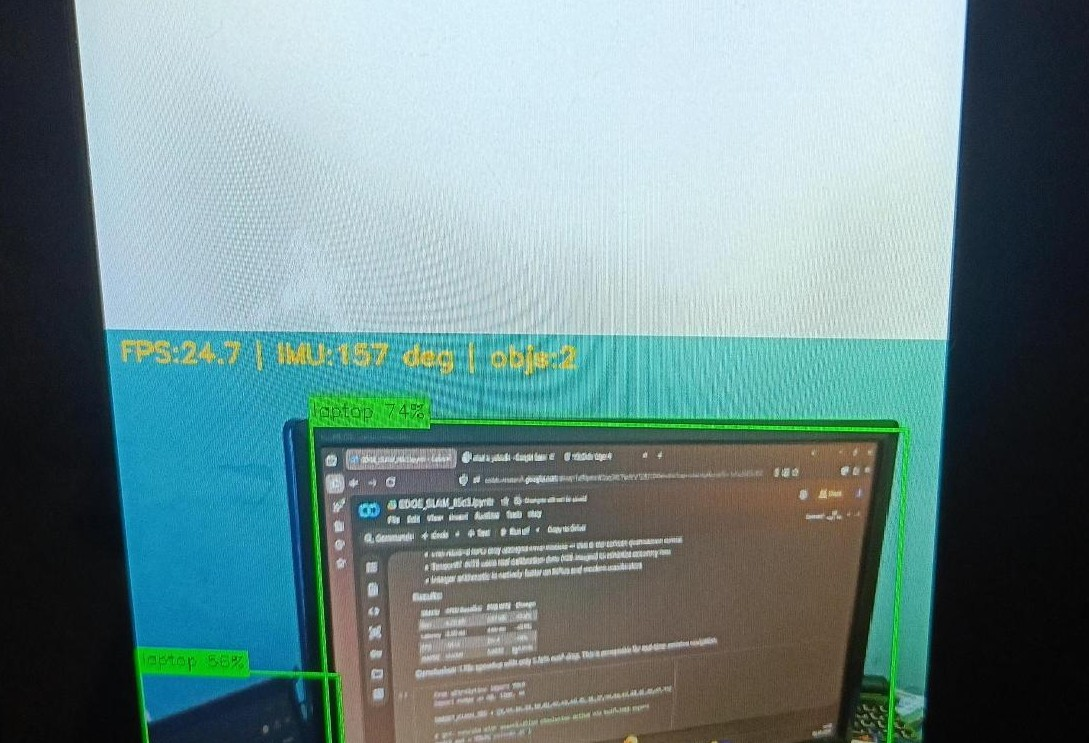
\includegraphics[width=\textwidth]{demo_detection_fps}
    \caption{Detection window: laptop detected at 24.7\,FPS with IMU heading 157°. Green bounding boxes with class labels and confidence scores are drawn on the live feed.}
    \label{fig:demo_fps}
  \end{subfigure}
  \hfill
  \begin{subfigure}[t]{0.48\textwidth}
    \centering
    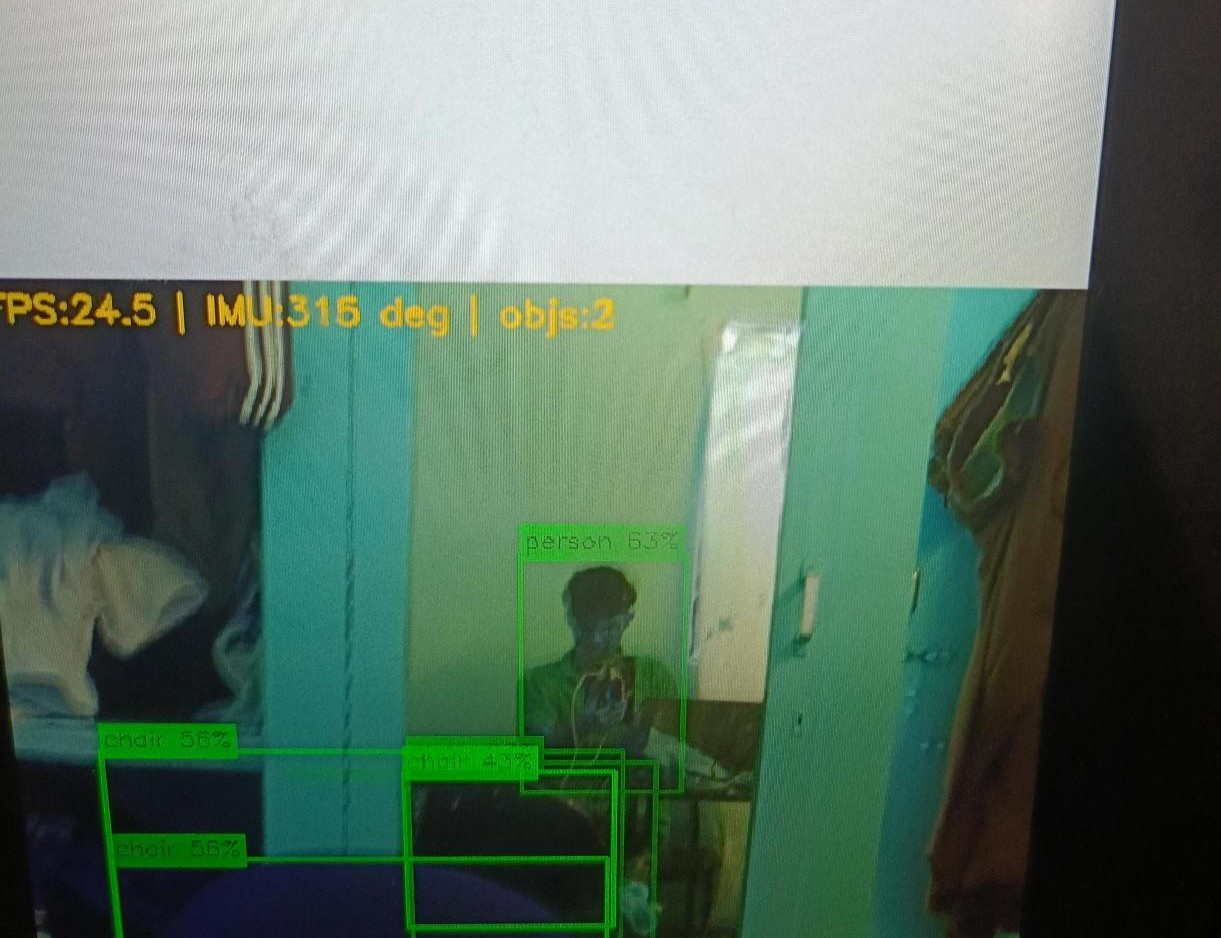
\includegraphics[width=\textwidth]{demo_detection_live}
    \caption{Detection window: person (63\%), three chair instances (56\%, 56\%, 43\%) detected simultaneously at IMU heading 315°. FPS sustained at 24.5.}
    \label{fig:demo_live}
  \end{subfigure}
  \caption{Window 1 — Live detection feed from the Pi Camera. The top overlay shows real-time FPS, IMU heading, and total object count each frame.}
  \label{fig:demo_detection}
\end{figure}

\begin{figure}[H]
  \centering
  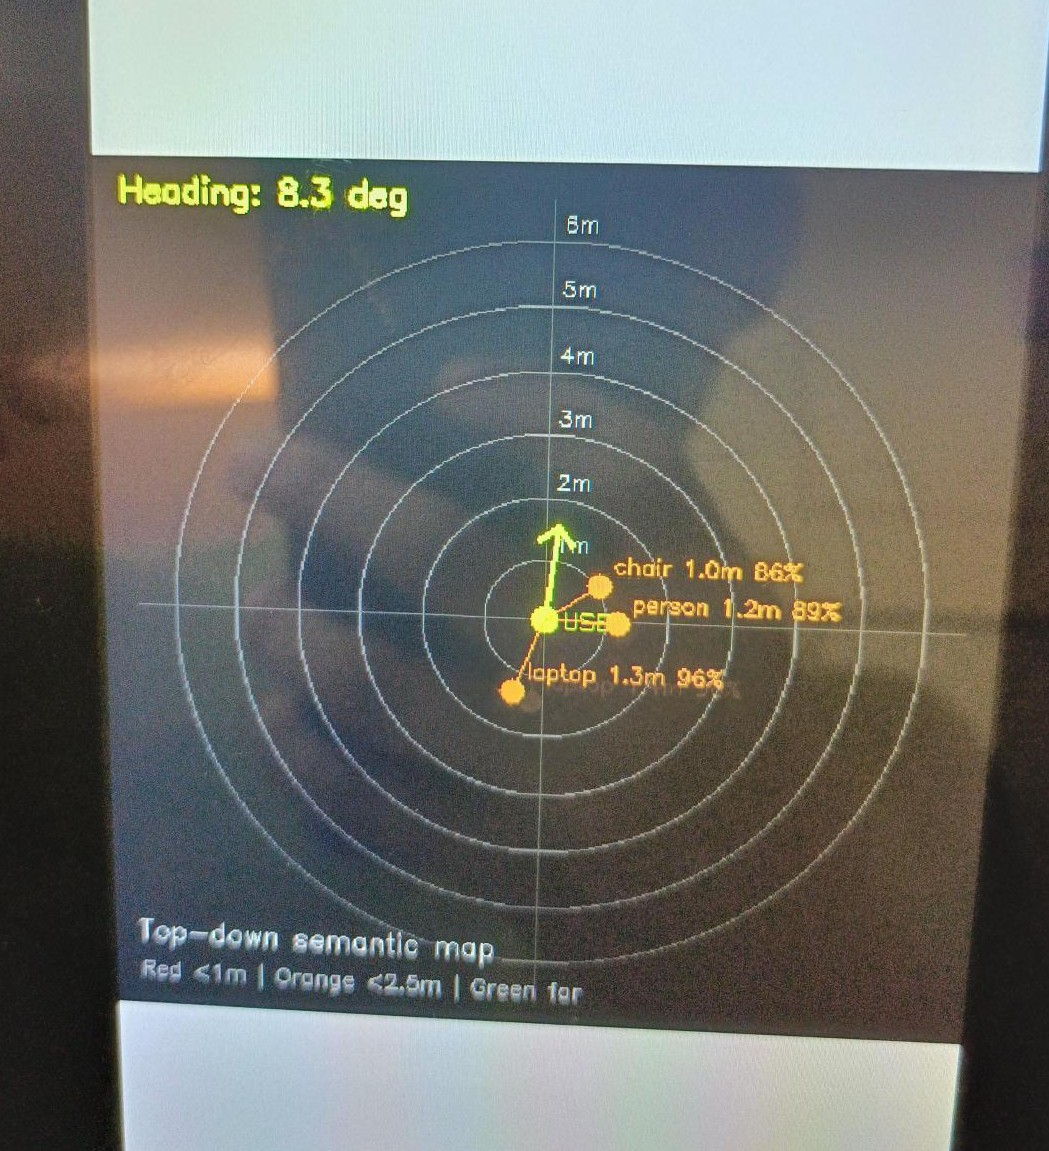
\includegraphics[width=0.52\textwidth]{demo_semantic_map}
  \caption{Window 2 — 2D top-down polar semantic map at IMU heading 8.3°. The user is at the center. Three objects are plotted at their estimated polar positions: chair at 1.0\,m (86\% confidence), person at 1.2\,m (89\%), and laptop at 1.3\,m (96\%). Range rings are at 1\,m intervals. Color coding: orange = within 2.5\,m, green = beyond 2.5\,m.}
  \label{fig:demo_map}
\end{figure}

\subsection{Observed Detections}

\begin{table}[H]
\centering
\caption{Sample Detections from the Live Demo Session}
\label{tab:detections}
\begin{tabular}{lccc}
\toprule
\textbf{Object} & \textbf{Confidence} & \textbf{Est.\ Distance} & \textbf{IMU Heading} \\
\midrule
chair  & 56\%, 56\%, 43\% & 1.0\,m & 315° \\
person & 63\%             & 1.2\,m & 315° \\
laptop & 74\%, 56\%       & 1.3\,m & 157° \\
\bottomrule
\end{tabular}
\end{table}

\subsection{Key Engineering Challenges}

\begin{table}[H]
\centering
\caption{Engineering Challenges and Resolutions}
\label{tab:challenges}
\begin{tabularx}{\textwidth}{lXX}
\toprule
\textbf{Challenge} & \textbf{Root Cause} & \textbf{Resolution} \\
\midrule
DFC incompatible with Colab GPU & DFC v3.33.1 uses CUDA libs incompatible with NVIDIA Blackwell (RTX 40xx) & Force CPU-only mode for the DFC optimize step \\
6-output Detect head & YOLOv8 DFL tensors cannot be absorbed by the DFC graph optimizer & Output 6 raw heads from HEF; decode DFL on RPi5 CPU \\
IMU handshake failure & Nicla resets on USB open, invalidating \texttt{NICLA\_IMU\_READY} signal & Poll directly for \texttt{A:<angle>} lines; no handshake dependency \\
ONNX opset mismatch & Default opset 13 uses ops unsupported by DFC & Re-export with \texttt{opset\_version=11} \\
\bottomrule
\end{tabularx}
\end{table}

% =============================================================================
\section{Conclusion}
\label{sec:concl}
% =============================================================================

We presented Edge-SLAM, a self-contained edge-AI system that runs real-time object detection and 2D semantic mapping on a Raspberry Pi 5 augmented with a Hailo-8 NPU. The five-stage compression pipeline produces a 4.5\,MB INT8 HEF that achieves \textbf{24.7\,FPS} on device and \textbf{+9.4\% mAP50} over the uncompressed FP32 baseline. The 2D polar map, updated each frame using gyroscope yaw from a Nicla Vision IMU, gives a clear visual snapshot of detected object positions relative to the user.

Key lessons from this project are:
\begin{enumerate}
  \item Hailo deployment requires going through the DFC — off-the-shelf INT8 models (TensorRT, TFLite) cannot run on Hailo-8.
  \item YOLOv8's DFL decode must stay on the host CPU; the DFC cannot fuse it into the HEF.
  \item Structured pruning \emph{before} INT8 quantization improved mAP — removing low-magnitude filters reduces activation noise that would otherwise be amplified by quantization.
  \item COCO128 is insufficient for effective QAT; the full COCO dataset would be needed.
  \item Gyroscope-only yaw integration drifts over time; a magnetometer or visual loop-closure correction would be needed for longer sessions.
\end{enumerate}

\noindent\textbf{Future directions} include replacing the reference-height distance heuristic with a lightweight monocular depth estimator, adding visual odometry for drift-free localization, and extending the map to 3D voxels using depth + IMU fusion.

% =============================================================================
\section*{Contributor Roles}
% =============================================================================

\begin{table}[H]
\centering
\caption{Team Contribution Breakdown}
\label{tab:contrib}
\begin{tabular}{llp{9.5cm}}
\toprule
\textbf{Name} & \textbf{SR No.} & \textbf{Contributions} \\
\midrule
Karney Jayanath & 26831 &
  Model training and optimization — YOLOv8n fine-tuning on COCO128, PTQ, QAT, L1 structured pruning, KD ablation, Colab training infrastructure, benchmark data collection and analysis \\
Shreevathsa K S & 25905 &
  RPi5 inference pipeline — Hailo HEF deployment, HailoRT integration, DFL post-processing decoder (\texttt{main\_RPI.py}), Picamera2 capture loop, NMS and bounding-box rendering \\
Rajneesh Babu & 26058 &
  2D semantic mapping — Nicla Vision IMU firmware (\texttt{main\_Nicla.py}), gyroscope bias calibration, dead-band filtering, IMU–RPi5 serial protocol, polar map construction, EMA smoothing, distance estimation \\
\bottomrule
\end{tabular}
\end{table}

% =============================================================================
\ifCLASSOPTIONcaptionsoff\newpage\fi

\begin{thebibliography}{10}

\bibitem{redmon2016you}
J.\ Redmon, S.\ Divvala, R.\ Girshick, and A.\ Farhadi,
``You Only Look Once: Unified, Real-Time Object Detection,''
\emph{Proc.\ IEEE CVPR}, pp.\ 779--788, 2016.

\bibitem{jocher2023yolov8}
G.\ Jocher, A.\ Chaurasia, and J.\ Qiu,
``Ultralytics YOLOv8,'' 2023.
[Online]. Available: \url{https://github.com/ultralytics/ultralytics}

\bibitem{hailo8}
Hailo Technologies,
``Hailo-8 AI Processor,'' 2023.
[Online]. Available: \url{https://hailo.ai/products/hailo-8}

\bibitem{lin2014microsoft}
T.-Y.\ Lin et al.,
``Microsoft COCO: Common Objects in Context,''
\emph{ECCV}, pp.\ 740--755, 2014.

\bibitem{jacob2018quantization}
B.\ Jacob et al.,
``Quantization and Training of Neural Networks for Efficient Integer-Arithmetic-Only Inference,''
\emph{Proc.\ IEEE CVPR}, pp.\ 2704--2713, 2018.

\bibitem{li2017pruning}
H.\ Li, A.\ Kadav, I.\ Durdanovic, H.\ Samet, and H.P.\ Graf,
``Pruning Filters for Efficient ConvNets,''
\emph{ICLR}, 2017.

\bibitem{hinton2015distilling}
G.\ Hinton, O.\ Vinyals, and J.\ Dean,
``Distilling the Knowledge in a Neural Network,''
\emph{arXiv:1503.02531}, 2015.

\bibitem{picamera2}
Raspberry Pi Ltd.,
``Picamera2 Library,'' 2023.
[Online]. Available: \url{https://datasheets.raspberrypi.com/camera/picamera2-manual.pdf}

\end{thebibliography}

\vfill
\end{document}
